% !TeX encoding = UTF-8
% !TeX spellcheck = es_AR
% arara: pdflatex
% arara: pdflatex
% arara: pdflatex
% arara: clean: {files: [03_html.aux, 03_html.out, 03_html.log]}
% arara: clean: {files: [03_html.fdb_latexmk, 03_html.fls, 03_html.vrb, 03_html.synctex.gz]}

%% Add the word "answers" to document class parameters in order to print the solutions.
\documentclass[12pt, addpoints]{../../common/epyl_exam_template}

\title{Práctica 1.3 - HTML}
\date{2018.1}

\begin{document}
\makeexamheader
\makeexamtitle
\examrule

\begin{questions}
  \question Utilizando HTML, diseñar en un archivo de texto una página
  que actuará como la portada del periódico ``El Sol''.
  \begin{parts}

  \part
    Agregue el título “Diario el Sol”, y luego dos subtítulos: “Noticias destacadas”
    y “Noticias deportivas”. Escriba un párrafo descriptivo para cada una de
    las secciones. El resultado debería ser similar al siguiente:

    \frame{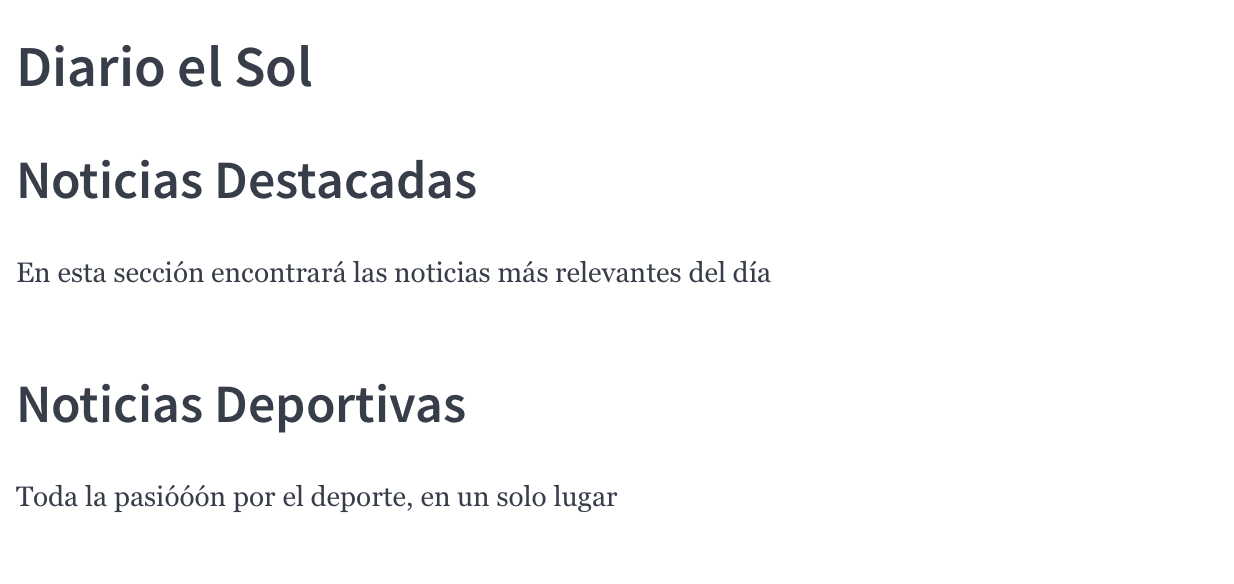
\includegraphics[scale=0.5]{img/markdown_paper_A.png}}
    \begin{solution}
      \begin{lstlisting}[language=HTML]
<!DOCTYPE html>
<html>
  <head>
    <meta charset="utf-8">
  <head>
  <body>
    <h1>Diario El Sol</h1>
    <h2>Noticias destacadas</h2>
    <p>En esta seccion encontrara las noticias mas
    relevantes del dia</p>
    <h2>Noticias deportivas</h2>
    <p>Toda la pasion por el deporte, en un solo lugar</p>
  </body>
</html>
      \end{lstlisting}
    \end{solution}

    \part
    Agregue tres noticias a cada sección del sitio anterior. Puede buscar
    noticias en un medio de su preferencia, o inventarlas. Cada noticia
    debe contar con título, de menor jerarquía que los de las secciones,
    y un copete (resumen de la noticia) en donde aparezcan algunas palabras
    o frases clave en negrita e itálica. El resultado debería ser similar al
    siguiente (la sección de noticias deportivas debería ser similar):

    \frame{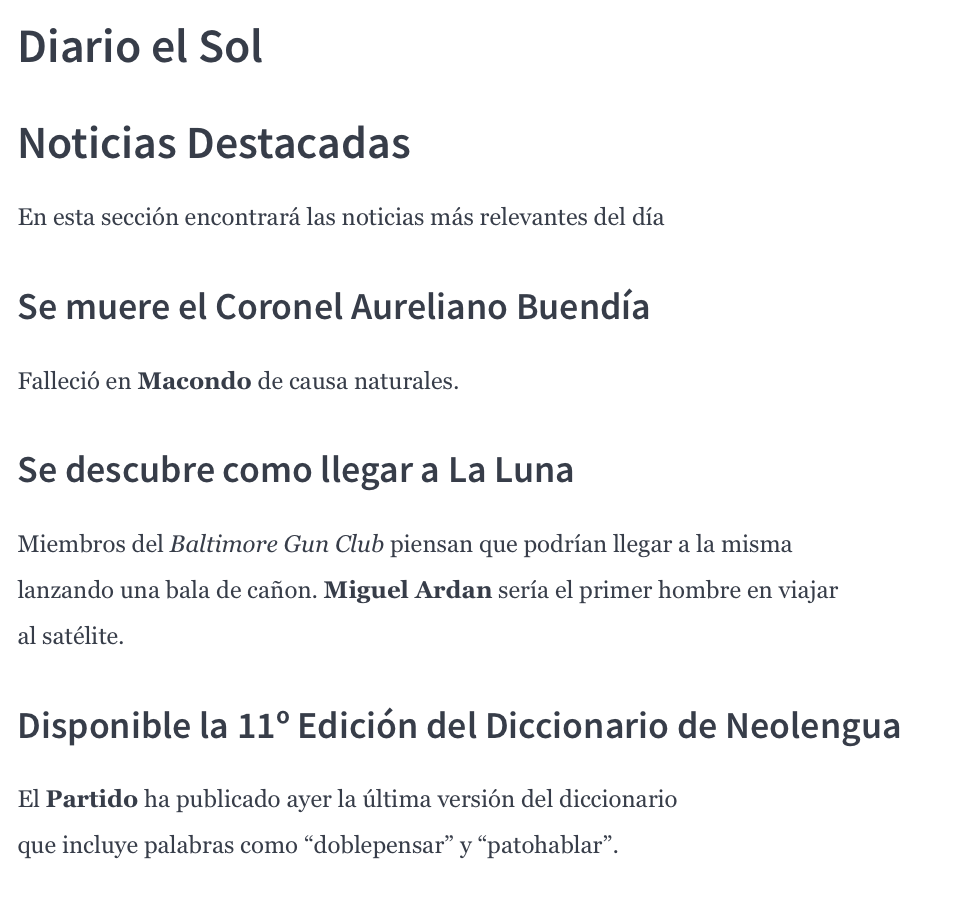
\includegraphics[scale=0.7]{img/markdown_paper_B.png}}

    \begin{solution}
      \begin{lstlisting}[language=HTML]
<!DOCTYPE html>
<html>
  <head>
    <meta charset="utf-8">
  <head>
  <body>
    <h1>Diario El Sol</h1>
    <h2>Noticias destacadas</h2>
    <p>En esta seccion encontrara las noticias mas
    relevantes del dia</p>

    <h4>Se muere el Coronel Aureliano Buendia</h4>
    <p>Fallecio en <strong>Macondo</strong> de causa
    naturales.</p>

    <h4>Se descubre como llegar a La Luna</h4>
    <p>Miembros del <em>Baltimore Gun Club</em> piensan que
    podrian llegar a la misma lanzando una bala de canon.
    <strong>Miguel Ardan</strong> seria el primer hombre en
    viajar al satelite.</p>

    <h4>Disponible la 11va Edicion del Diccionario de
    Neolengua.</h4>
    <p>El <strong>Partido</strong> ha publicado ayer la
    ultima version del diccionario que incluye palabras como
    "doblepensar" y "patohablar".</p>

    <h2>Noticias deportivas</h2>
    <p>Toda la pasion por el deporte, en un solo lugar</p>

    <!-- ... -->
  </body>
</html>
    \end{lstlisting}
  \end{solution}

    \part
    Si no lo ha hecho antes, utilice las etiquetas semánticas para separar
    el contenido del sitio y aseguresé de indentar correctamente su código.

    \begin{solution}
      \begin{lstlisting}[language=HTML]
<!DOCTYPE html>
  <!-- ... -->
  <body>
    <header>
      <h1>Diario El Sol</h1>
    </header>
    <section>
      <header>
        <h2>Noticias destacadas</h2>
        <p>
          En esta seccion encontrara las noticias
          mas relevantes del dia
        </p>
      </header>

      <article>
        <h4>Se muere el Coronel Aureliano Buendia</h4>
        <p>
          Fallecio en <strong>Macondo</strong>
          de causa naturales.
        </p>
      </article>

      <article>
        <h4>Se descubre como llegar a La Luna</h4>
        <p>
          Miembros del <em>Baltimore Gun Club</em>
          piensan que podrian llegar a la misma lanzando
          una bala de canon. <strong>Miguel Ardan</strong>
          seria el primer hombre en viajar al satelite.
        </p>
      </article>

      <article>
        <h4>Disponible la 11va Edicion del Diccionario de
        Neolengua.</h4>
        <p>
          El <strong>Partido</strong> ha publicado ayer la
          ultima version del diccionario que incluye
          palabras como "doblepensar" y "patohablar".
        </p>
      </article>
    </section>

    <section>
      <header>
        <h2>Noticias deportivas</h2>
        <p>
        Toda la pasion por el deporte, en un solo lugar
        </p>
        <!-- ... -->
  </body>
</html>
    \end{lstlisting}
  \end{solution}

    \part
    Agregar el link de referencia a los sitios de donde tomo las noticias
    (o coloque un enlace a sitios de su preferencia si inventó las noticias)
    con el texto ``Leer más''. El resultado debería ser (obviando las líneas
    horizontales):

    \frame{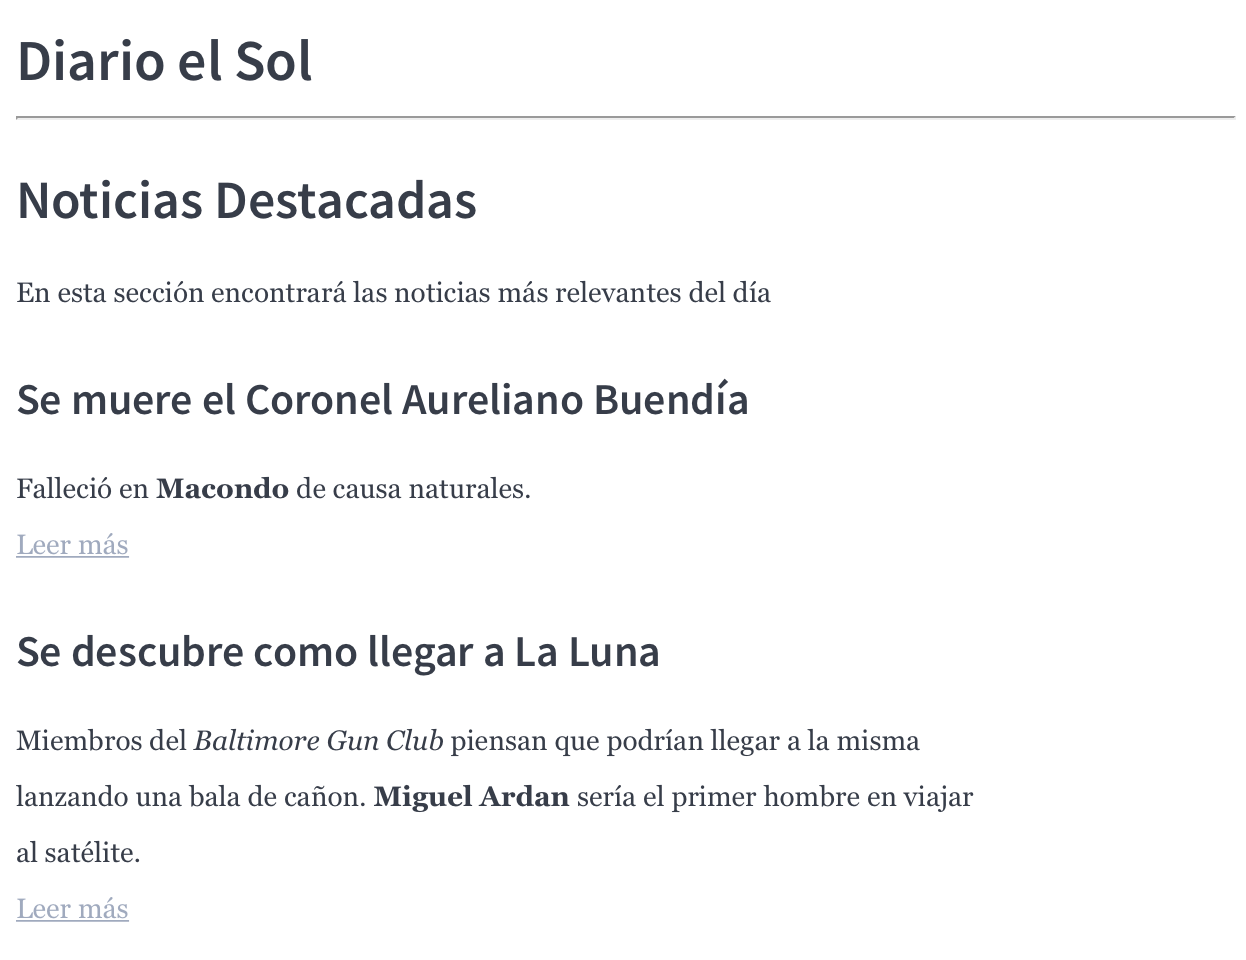
\includegraphics[scale=0.7]{img/markdown_paper_D.png}}

    \begin{solution}
      \begin{lstlisting}[language=HTML]
<!DOCTYPE html>
    <!-- ... -->
      <article>
        <h4>Se muere el Coronel Aureliano Buendia</h4>
        <p>
          Fallecio en <strong>Macondo</strong>
          de causa naturales.
        </p>
        <p>
          <a href="https://amazon.es/
                Cien-anos-de-soledad">Leer mas</a>
        </p>
      </article>
    <!-- ... -->
    \end{lstlisting}
  \end{solution}

  \part
  Agregar, antes del título del diario, la imagen del logo del mismo.
  Puede utilizar el logo que guste tomandolo de internet. El resultado debe
  ser similar a:

  \frame{
\includegraphics[scale=0.7]{img/markdown_paper_E.png}}

  \begin{solution}
    \begin{lstlisting}[language=HTML]
<!DOCTYPE html>
  <!-- ... -->
  <body>
    <header>
      <img src="http://www.elsolnoticias.com.ar/
                imagenes/elsolquilmes.png">
      <h1>Diario El Sol</h1>
    </header>
    <section>
      <header>
        <h2>Noticias destacadas</h2>
        <p>
          En esta seccion encontrara las noticias
          mas relevantes del dia
        </p>
      </header>
      <!-- ... -->
    \end{lstlisting}
  \end{solution}

  \part
  Agregar justo despues del título, y previo a la primer sección, un listado
  con todas las secciones del diario. Las mismas son: Sociedad, Politica,
  Policiales, Deportes, Economía y Cultura. El resultado debe ser como el
  siguiente:

  \frame{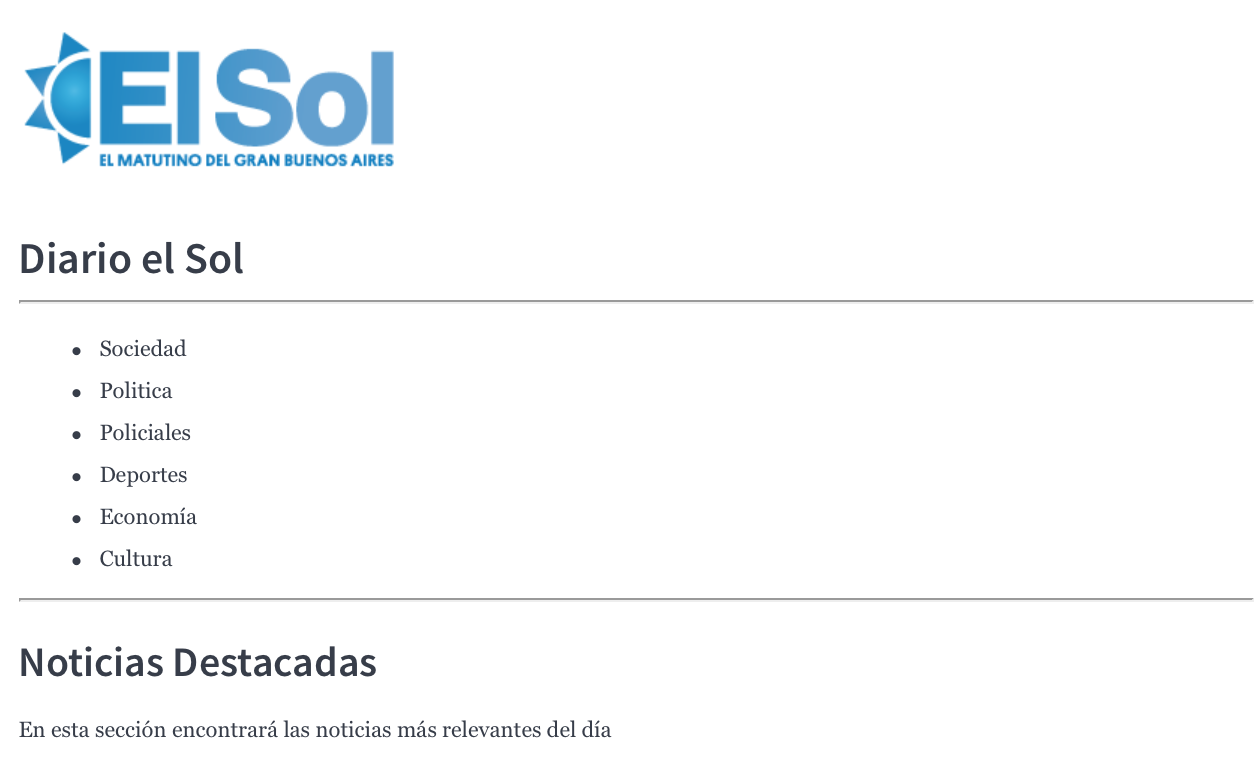
\includegraphics[scale=0.7]{img/markdown_paper_F.png}}

  \begin{solution}
    \begin{lstlisting}[language=HTML]
<!DOCTYPE html>
  <!-- ... -->
  <body>
    <header>
      <img src="http://www.elsolnoticias.com.ar/
                imagenes/elsolquilmes.png">
      <h1>Diario El Sol</h1>
      <nav>
        <ul>
          <li>Sociedad</li>
          <li>Politica</li>
          <li>Policiales</li>
          <li>Deportes</li>
          <li>Economia</li>
          <li>Cultura</li>
        </ul>
      </nav>
    </header>
    <!-- ... -->
    \end{lstlisting}
  \end{solution}

\end{parts}

  \question
    Dados los siguientes párrafos en HTML, resaltar en negrita los sujetos, y en
    cursiva los verbos.
    \begin{quoted}
      <p>
        La ley de Moore expresa que aproximadamente cada dos años se duplica el
        número de transistores en un microprocesador.
      </p>
      <p>
        La consecuencia directa de la ley de Moore es que los precios bajan al
        mismo tiempo que las prestaciones suben. Así, la computadora que hoy
        vale 3000 dólares costará la mitad al año siguiente y estará obsoleta en
        dos años. En 26 años el número de transistores en un chip se ha
        incrementado 3200 veces.
      </p>
    \end{quoted}

  \question
    Buscar en internet la receta para hacer tallarines caseros, y redactarla
    prolijamente en un documento HTML. Utilizar una lista no ordenada para
    los ingredientes, y una lista ordenada para los pasos a seguir.

  \question
    Elaborar una tabla de doble entrada en donde, como columnas, se tengan los
    diferentes años (desde 1985 a 2015) y como fila los siguientes 5 paises:
    (Argentina, Brasil, Estados Unidos, España, Suecia). Como datos, en cada
    celda se deben colocar los datos del Indice de Desigualdad Social, o Indice
    GINI elaborado por el Banco Mundial.
    \\
    \textit{Puede buscar los datos en:\\
      \hyperref[https://datos.bancomundial.org/indicador/SI.POV.GINI?locations=AR]
      {https://datos.bancomundial.org/indicador/SI.POV.GINI?locations=AR}
    }

  \question
    Realizar un dibujo (esquema) en donde se muestre el resultado del
    siguiente código HTML tras al ser vidsualizado en un navegador.\\~\\
    \textit{El objetivo es realizar el dibujo previo a visualizarlo, pero
    puede copiar el código en un archivo y abrirlo con el navegador para
    contrastar su respuesta con el resultado real. Si no sabe que efecto
    tiene un atributo, o no conoce una etiqueta, busque información sobre
    ella en Internet}.

    \begin{lstlisting}[language=HTML]
<!DOCTYPE html>
<html>
<head>
  <meta charset="utf-8">
  <title>El Proyecto FreeBSD</title>
</head>
<body>
<body>
  <header>
    <h2 class="blockhide">Cabecera y Logo</h2>
    <div id="headerlogoleft">
      <a href="." title="FreeBSD">
        <img src="./../layout/images/logo-red.png"
        width="457" height="75" alt="FreeBSD">
      </a>
    </div>
    <div id="headerlogoright">
      <h2 class="blockhide">Enlaces externos</h2>
      <nav>
        <ul id="SEARCHNAVLIST">
          <li>
            <a href="./../donations/">Donaciones</a>
          </li>
          <li class="last-child">
            <a href="./mailto.html">Contactar</a>
          </li>
        </ul>
      </nav>
    </div>
  </header>
  <section>
    <h1>Basado en BSD UNIX</h1>
    <p>
      FreeBSD es un avanzado sistema operativo para
      arquitecturas x86 compatibles (como <em>Pentium</em>
      y <em>Athlon</em>), amd64 compatibles (como
      <em>Opteron</em>, <em>Athlon 64</em>, <em>EM64T</em>),
      <em>UltraSPARC</em>, <em>IA-64</em>, <em>PC-98</em> y
      <em>ARM</em>.
		<p>
    <p>
      FreeBSD es un derivado de BSD, la version de
			UNIX desarrollada en la <strong>Universidad
			de California, Berkeley</strong>. FreeBSD es
      desarrollado y mantenido por un
			<a href="./../contributors/index.html">
			numeroso equipo de personas</a>. El soporte para
      otras
			<a href="./platforms/index.html">arquitecturas</a>
			esta en diferentes fases de desarrollo.
    </p>
  </section>
  <section>
    <h2><a href="./../releases/">ULTIMAS VERSIONES</a></h2>
    <ul id="FRONTRELEASELIST">
      <li>
        <a href="./../releases/11.1R/announce.html">
          Release estable: 11.1
        </a>
      </li>
      <li>
        <a href="./../releases/10.2R/announce.html">
          Release estable (heredera): 10.2
        </a>
      </li>
      <li>
        <a href="./../where.html#helptest">
          Proxima Release 10.4 - BETA1
        </a>
      </li>
    </ul>
  </section>
  <footer>
    <p>
      <a href="https://www.freebsd.org/es/search/index-site.html">
        Mapa del sitio
      </a>
      |
      <a href="https://www.freebsd.org/es/copyright/">
        Noticias del Copyright
      </a>
      | 1995-2010 El Proyecto FreeBSD.
      Quedan reservados todos los derechos.
    </p>
    <p>
      Last modified: 2014-03-03
    </p>
  </footer>
</body>
</html>
    \end{lstlisting}

  \question
    Realizar su Currículum Vitae utilizando HTML. Agregar una foto,
    datos de contacto, links de referencias a las empresas donde haya
    trabajado, etc. Agregue también una carta de presentación personal
    junto con el CV y enlace ambas páginas.

\end{questions}

\end{document}
